\documentclass{article}

% if you need to pass options to natbib, use, e.g.:
%     \PassOptionsToPackage{numbers, compress}{natbib}
% before loading neurips_2019

% ready for submission
% \usepackage{neurips_2019}

% to compile a preprint version, e.g., for submission to arXiv, add add the
% [preprint] option:
\usepackage[preprint]{neurips_2019}
\bibliographystyle{unsrt}

% to compile a camera-ready version, add the [final] option, e.g.:
%     \usepackage[final]{neurips_2019}

% to avoid loading the natbib package, add option nonatbibnatbib:
%     \usepackage[nonatbib]{neurips_2019}

\usepackage[utf8]{inputenc} % allow utf-8 input
\usepackage[T1]{fontenc}    % use 8-bit T1 fonts
\usepackage{hyperref}       % hyperlinks
\usepackage{url}            % simple URL typesetting
\usepackage{booktabs}       % professional-quality tables
\usepackage{amsfonts}       % blackboard math symbols
\usepackage{nicefrac}       % compact symbols for 1/2, etc.
\usepackage{microtype}      % microtypography
\usepackage{graphicx}
\usepackage{titlesec}
\usepackage{hyperref}
\usepackage{enumitem}
\usepackage{lmodern}
\usepackage{amsmath}
\usepackage{fancyhdr}
\usepackage{textcomp}
\usepackage{lmodern}% http://ctan.org/pkg/lm
\usepackage[table,x11names,svgnames]{xcolor}
\usepackage{soul}
\usepackage{parskip}
\usepackage{multirow}
\usepackage{array}
\usepackage{afterpage}
\usepackage{tabularx}
\usepackage{float}
\usepackage{placeins}
\usepackage{tablefootnote}
\usepackage{microtype}
\usepackage{textcomp}
\usepackage{titlesec}
\usepackage{enumitem}
\usepackage{listings}
\usepackage{subcaption}
\usepackage{verbatim}
\usepackage[htt]{hyphenat}
\usepackage[linesnumbered, noline, noend]{algorithm2e}

% optimization
\DeclareMathOperator*{\argmin}{arg\,min}
\DeclareMathOperator*{\argmax}{arg\,max}


\title{Learn to play Go}

\author{%
  Albert Liu \\
  Department of Computer Science\\
  Stanford University\\
  \texttt{albertpl@stanford.edu} \\
}

\begin{document}

\maketitle

\section{Infrastructure}
As illustrated in Figure \ref{fig:env}, our simulator includes a Go gameplay engine, which is based on Pachi \cite{baudivs2011pachi}, an open source Go framework. We choose Pachi due to its efficiency and simple APIs. Each agent is given a 2D numpy array (e.g. $19 \times 19$), representing current board with each element encoding the color of stone, 0 for empty, 1 for black stone and 2 for white stone. Then each agent returns the next move to play, encoded as position of the board (e.g. E4) and a pass action. 
Each agent can optionally persist the game records, numpy arrays that hold the board representation, moves and etc., to disk, which are used as experiences for the reinforcement learning agents. We use Keras as our deep learning framework. 

\section{Approach}
Minimax search or AlphaBeta search is intractable due to enormous search space. Instead, we start with Monte Carlo Tree Search \cite{coulom2006efficient}. Then we explore policy gradient based methods. Finally we will combine tree search and function approximation approach, following AlphaGoZero \cite{silver2017masteringalphagozero}.  But first, we discuss the baseline and oracle.

\subsection{Baseline}
For baseline, we write a random agent which selects legal move randomly, except that it won't commit suicide, i.e. filling in its own eye, which is an empty position where all adjacent positions and three out of four diagonally adjacent positions are its stones (or edges).

\subsection{Oracle}
We use Pachi built-in \textit{UCT} engine as our oracle which is said to achieve highest amateur expect level (KGS 7 dan) on $9 \times 9$ or KGS 2d rank on reasonable hardware, where dan is expert Go ranking, from 1 to 7 (low to high). Technically the \textit{UCT} engine implements RAVE \cite{gelly2007combining}, instead of classic UCT. This engine incorporates lots of heuristics and predefined patterns above the basic Go rules, e.g. self-atari detector and ladder testing \cite{baudivs2011pachi}.

\subsection{Monte Carlo Tree Search}
The MCTS evaluate each node of the game tree by simulating random games. Each node $s$ is a game state, consisting of a tuple of (board representation, the player to play). And there is an edge between $s$ and $s'$ if and only if for some move $a$, $s' = \text{Succ}(s, a)$, where $\text{Succ}(s,a)$ is function that returns the next game state $s'$ after playing the move $a$. For each edge $(s, a)$, we maintain visit count $n(s,a)$ and value $q(s,a)$
\begin{algorithm} 
  \DontPrintSemicolon
  \caption{MCTS with UCB policy}
  \KwIn{root node $s_0$: current game state}
  \KwIn{$c>0$: parameter to control the degree of exploration}
  \While {within computation bound} {
    $ s \gets s_0 $ \\
    $ \Delta \gets \emptyset$ \\
    // selection based on tree policy: Upper Bound Confidence \\
    \While {$s$ is in the tree} {
      $a  \gets \argmax \{ q(s, a) + c \sqrt{\frac{\log \sum_{a'}n(s, a')}{n(s,a)}}$ \}\\
      $\Delta \gets \Delta \cup \{(s, a)\}  $ \\
      $s \gets \text{Succ}(s, a) $\\
    }
    expand tree to add $s$ \\
    simulate a random game from $s$ and let $r$ be the reward \\
    // update each node on the trajectory within the tree \\
    \For {$s, a \in \Delta $ } {
      $ n(s, a) \gets n(s,a) + 1 $ \\
      $ q(s, a) \gets q(s,a) +  \frac{1}{n(s,a)} (r - q(s,a))$ \\
    }
  }
\end{algorithm}

\subsection{Self-play}
In order to apply reinforcement learning, we need to collect experiences (i.e. game records). The standard approach is to have agents play against themselves and save the game records. We record the board position at each step perceived by the player, the move of the player, the color of the player, the final reward (-1 if white player wins, +1 if black player wins) and network predictions. Then later the agent can use these experiences to update its network.

\subsection{Actor-critic with baseline}
The policy gradient based methods, such as REINFORCE [TODO] and actor-critic [TODO], allow us to learn stochastic policy naturally. For our episodic cases, we define the objective function, $J(\theta)$, to be the start value of any state $S$, following our parameterized policy function $\pi_{\theta}$ which is approximated by a deep neural network, i.e.,  $J(\theta) = V_{\pi_{\theta}}(S)$. By Policy Gradient Theorem [TODO], we can compute the gradient as
$$ \nabla_{\theta} J(\theta) =  \mathbb E_{\pi_{\theta}} [ 
Q_{\pi_{\theta}}(S_t, A_t)] 
\nabla_{\theta} \log \pi_{\theta}(A_t|S_t) 
$$

REINFORCE method uses Monte Carlo method to give unbiased sample $G_t$ for $Q_{\pi_{\theta}}(S_t, A_t)]$ and the update rule is
$$ \theta_{t+1} = \theta_{t} + \alpha 
G_t 
\nabla_{\theta} \log \pi_{\theta}(A_t|S_t) 
$$
But Monte Carlo gradient typically has high variance and produces slow learning. Actor-critic with baseline is suggested [TODO] to solve such high variance issue. Let advantage function $
A_{\pi_{\theta}}(S_t, A_t) 
= 
Q_{\pi_{\theta}}(S_t, A_t)  - 
V_{\pi_{\theta}}(S_t) 
$, the update rule is
$$ \theta_{t+1} = \theta_{t} + \alpha 
A_{\pi_{\theta}}(S_t, A_t) 
\nabla_{\theta} \log \pi_{\theta}(A_t|S_t) 
$$

\subsection{Tree Search guided with NN}

\section{Error analysis}
\subsection{Monte Carlo Tree Search}
Here are our results for MCTS approach against baseline and oracle.
\begin{table}
  \caption{Results: MCTS}
  \label{tbl:mcts}
  \centering
  \begin{tabular}{c | c | c | c}
    opponent policy    &  number of rollouts per move & win rate  & median time per episode \\
    \hline
    random            &  100 &  0.92  & 2.4 \\
    random            &  1000 &  0.99  & 29.3 \\
    pachi \textit{UCT} engine  &  1000 &  0.16  & 35.1 \\
  \end{tabular}
\end{table}

We see our MCTS result gets better with more rollouts per move, as expected. But it still loses more games against pachi \textit{UCT} engine. And we speculate that reasons are
\begin{itemize}
  \item
    Rollout policy 

    Unlike our MCTS, pachi entails more Go knowledge when selecting next move during the game simulation. This is called \textbf{heavy} or strong rollout policy, whereas ours is called light rollout policy. Pachi's rule based simulation policy is handcrafted to mix in heuristics such as,  if the last move has put its own group in \textit{atari} we capture it; \textit{Nakade}a move is played inside the eyeshape to prevent the opponent from splitting it into two eyes \cite{baudivs2011pachi}.

  \item
    Priors
  
    We expand a new node by randomly selecting a legal move. But Pachi apply again a set of heuristic function to this decision, equivalently adding a prior probability distribution.  Specifically it takes the progressive bias strategy \cite{gelly2007combining}, which adds virtual simulations based on the applied heuristics with decreasing weights as the nodes are explored.

  \item
    RAVE 

    MCTS updates values of nodes with the reward of the simulation, along the sampled path from root to the leaf. But RAVE \cite{gelly2007combining} distributes the update to larger set of nodes. Basically it applies AMAF heuristics \cite{bouzy2004monte} (all-move-as-first), which keep previous simulations and apply it whenever we examine the same $(s, a)$ edge and then combines it with regular simulations.


    We believe the tree search guided by NN is a better approach. The NN is used to approximate an evaluation function and prior distributions.


\end{itemize}


\section{Figures, tables, references}
\subsection{Figures}
\begin{figure}
\centering
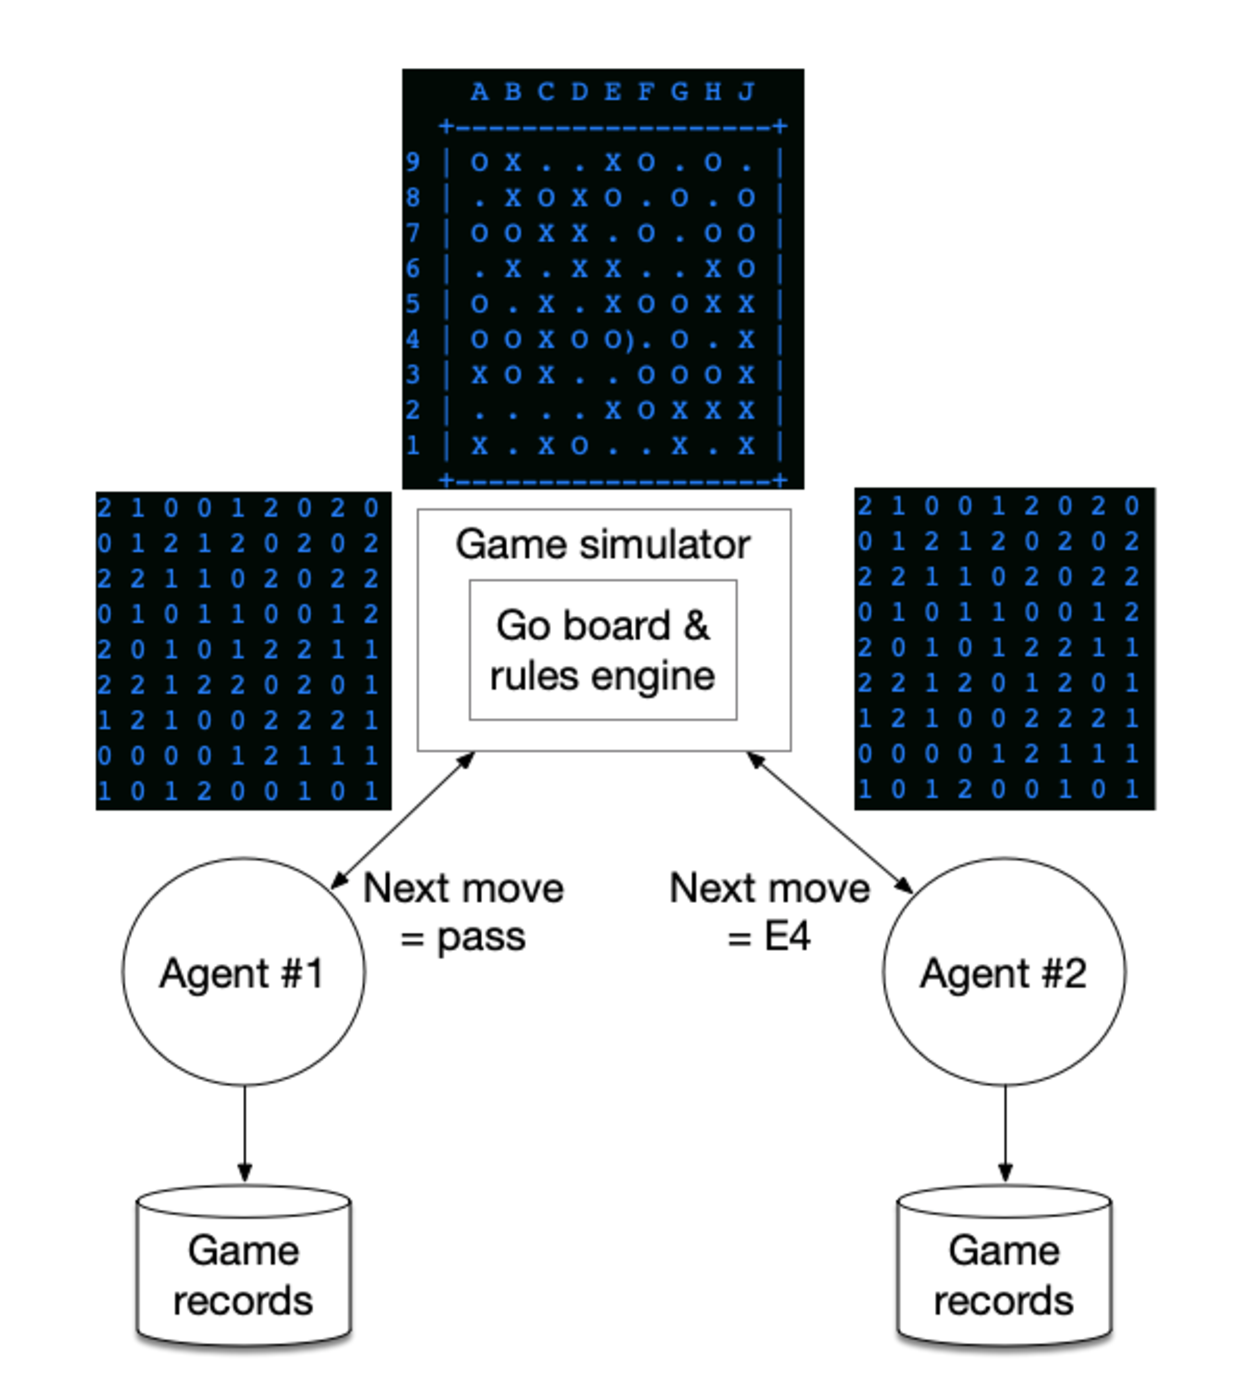
\includegraphics[width=0.8\linewidth]{simulator}
\caption{Environment setup}
\label{fig:env}
\end{figure}

\bibliography{reference} 

\end{document}
